\documentclass[12pt,compress,english,utf8,t]{beamer}

\usepackage{etex}

\usepackage[english]{babel}

\usepackage{tikz}
\usepackage{booktabs}
\usepackage{ragged2e}

\usepackage[protrusion=true,expansion=false]{microtype}

\title{Pugs, an experimental Perl 6 platform: a retrospective}
\author[Augsburg.pm]{
  \vspace{-1em} \\
  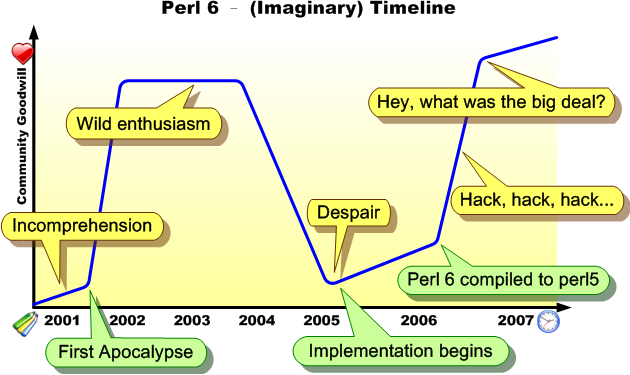
\includegraphics[scale=0.32]{images/timeline} \\[0.5em]
  Ingo Blechschmidt \\
  \texttt{<iblech@web.de>} \\
  {\scriptsize March ??th, 2015}
}
\date{March ??th, 2015}

\usetheme{Warsaw}
\usecolortheme{seahorse}
\definecolor{mypurple}{RGB}{100,0,255}
\setbeamercolor{structure}{fg=mypurple}
\usefonttheme{serif}
\usepackage{mathpazo}
\useinnertheme{rectangles}
\setbeamercovered{invisible}

\setbeamertemplate{title page}[default][colsep=-1bp,rounded=false,shadow=false,bg=white]
\setbeamertemplate{frametitle}[default][colsep=-2bp,rounded=false,shadow=false,center]

\setbeamertemplate{navigation symbols}{}
\setbeamertemplate{headline}{}

\newcommand*\oldmacro{}%
\let\oldmacro\insertshorttitle%
\renewcommand*\insertshorttitle{%
  \oldmacro\hfill\insertframenumber\,/\,\inserttotalframenumber\hfill}

\newcommand{\hil}[1]{{\usebeamercolor[fg]{item}{\textbf{#1}}}}

\newcommand{\atpos}[4]{%
  \begin{tikzpicture}[remember picture, overlay]%
    \node[anchor=south east] at (current page.south east) {#1};
  \end{tikzpicture}%
}

\newcommand{\centeredpar}[1]{%
  \begin{center}
    \parbox{0.9\textwidth}{%
      #1%
    }%
  \end{center}%
}

\newcommand{\sourcedquote}[4]{%
  ``#1''\par%
  {\raggedleft -- #2, #3, \href{#4}{link}\par}%
}

% Gonzalo Medina, http://tex.stackexchange.com/a/228198
\makeatletter
\def\Mdescription#1{%
  \advance\beamer@descdefault by \labelsep%
  \list
  {}
  {\labelwidth\beamer@descdefault%
  \leftmargin\beamer@descdefault%
  \let\makelabel\beamer@descriptionitem
  \settowidth\labelwidth{\beamer@descriptionitem{#1}}%
  \setlength\leftmargin{\labelwidth}% 
  \addtolength\leftmargin{\labelsep}%
  }%
  \beamer@cramped%
  \raggedright
  \beamer@firstlineitemizeunskip%
}
\def\endMdescription{\ifhmode\unskip\fi\endlist}
\long\def\beamer@descriptionitem#1{%
  \def\insertdescriptionitem{#1}%
  {\usebeamertemplate**{description item}}\hfil}
\makeatother

\setbeameroption{show notes}

\begin{document}

\frame{\titlepage}

\frame[plain]{\justifying
  \textbf{Abstract.}
  ``Hi. Today I have started working on specifying and implementing
  Featherweight Perl 6 (FP6), a side-effect-free subset of Perl~6.''
  Audrey Tang used these words to unveil the Pugs project in February of 2005.
  Initially conceived as an implementation of a small subset of Perl~6 in
  Haskell, the project quickly grew to contain a full-fledged compiler and
  interpreter for Perl~6 and drew a large and diverse community.

  \medskip
  The talk will give a subjective survey of the history of Pugs. We will pay
  particular attention to the special manner with which Audrey Tang led the project and
  what the philosophy ``-Ofun'' meant to the developers. We'll also discuss
  which parts of Pugs were absorbed into other implementations of Perl~6 and
  which influence Pugs had on the Perl and Haskell communities.
  \medskip

  \textbf{Warning.} The account is mostly from memory and not properly
  researched. Do not trust it!
  \par
}

\frame{\tableofcontents}

\section{Timeline of Pugs development}

\subsection{The beginning}
\logo{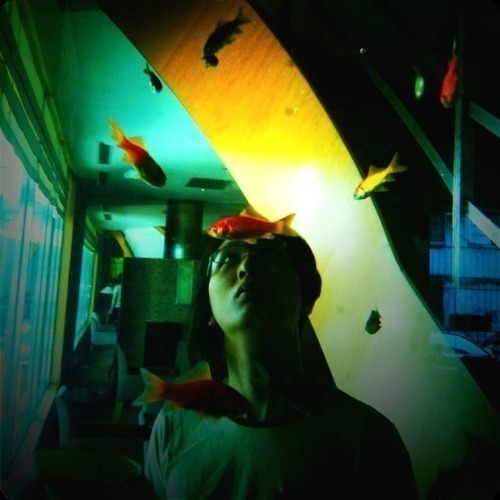
\includegraphics[scale=0.15]{images/audreyt}}
\begin{frame}\frametitle{The beginning}
  \centeredpar{
    \hil{``Hi. Today I have started working on specifying and implementing
    Featherweight Perl 6 (FP6), a side-effect-free subset of Perl~6.''}

    \raggedleft -- Audrey Tang, February 2nd, 2005
  }

  \only<1>{
    \begin{Mdescription}{2001}
      \item[2001] Apocalypse 1
      \item[2004] Many Apocalypse and Synopse documents
      \item[2005] Active discussion on perl6-language@perl.org
      \item[2005] Pugs, providing the first implementation
      \item[]
      \item[2005] Facebook
      \item[2005] YouTube
      \item[2008] GitHub
    \end{Mdescription}
  }

  \only<2->{
    \begin{itemize}
      \item Audrey's first post contained a language semantics question.
      \item Important insight: Specification and implementation have to be
      developed hand in hand.
    \end{itemize}
  }
\end{frame}

% Show first screenshot of Pugs

\note{
  \begin{itemize}
    \justifying
    \item \sourcedquote{As I'm finding my way through TaPL and ATTaPL today, it occurs to me that
    I should implement a real language as an exercise; that real language turns
    out to be Perl~6. So it begins \ldots}{Audrey Tang}{February 1st,
    2005}{http://wayback.archive.org/web/20050206202119/http://use.perl.org/~autrijus/journal/}
    \item TaPL refers to \emph{Types and Programming Languages}, a
    computer-science book on implementing programming languages.
    \item Actually, there was an implementation before Pugs. Namely, a small
    project sitting in the Parrot source tree.
  \end{itemize}
}

% Day 14: Testing framework
% Day 23: Test.pm flies

\appendix

\note{
  \begin{itemize}
    \justifying
    \item \sourcedquote{One of my goals of this project is to keep it dual-cultured. So the
    source tree is managed with bth svk and darcs; the build system requires
    both Perl5 and GHC; I will submit my Apocrypha series of design documents
    as monthly articles to both Perl.com and The Monad Reader; the project info
    is on both CPAN and the Haskell Wiki; etc, etc.}{Audrey Tang}{February 6st,
    2005}{http://wayback.archive.org/web/20050206202119/http://use.perl.org/~autrijus/journal/}

    \item Foreshadowing node.js:
    \sourcedquote{Indeed, if JavaScript2 does survive the standardization
    process, it is entirely possible that it may become the next Ruby, because
    writing programs that runs at both client and server side is a strong
    motivation -- the same reason to keep Pugs targetable to multiple
    backends.}{Audrey Tang}{October 30th,
    2005}{http://wayback.archive.org/web/20060924085336/http://use.perl.org/journal.pl?op=display&uid=1505&start=10}

    \item \sourcedquote{In other news, Pugs was mentioned on The Haskell
    Sequence today. Indeed, I have noted that a significant part of questions
    asked in #haskell are from camelfolks. Conversely, we saw a large influx
    from lambdafolks to #perl6 as well. Lots of knowledge transfer is
    happening, which makes me really happy.}{Audrey Tang}{February 24th,
    2005}{http://pugs.blogs.com/pugs/2005/02/day_24_an_amazi.html}
  \end{itemize}
}

\end{document}

http://www.slideshare.net/autang/pugs-a-perl-6-implementation
http://www.slideshare.net/autang/ofun-optimizing-for-fun
